\subsection{P1 Internal Verification and Numerical Convergence}
The verification suite tests implementation consistency and known limiting solutions; no flight-data validation is claimed. Standard-atmosphere base pressures at 0, 11, 20, 32, and 47 km geopotential altitude agree with rounded reference values within $4.8\times10^{-6}$ relative error. Out-of-range atmospheric queries are rejected. A vertical vacuum coast conserves the modeled specific mechanical energy to $7.5\times10^{-9}$ J/kg over 20 s. Constant-thrust mass history and horizontal ideal-rocket velocity agree with their analytic expressions to $7.6\times10^{-10}$ kg and $2.9\times10^{-14}$ m/s, respectively, in the chosen tests. These small residuals apply to those tests and do not measure real-world accuracy.

Pure axial and pure crossflow force limits, static pressure-center torque, torque-free rotation, damping sign, gimbal sign, and air-relative dissipativity are checked. For pure centered rotation, Eq.~\eqref{eq:rotation} provides an independent integral. Midpoint-strip relative errors are 2\%, 0.5\%, 0.125\%, 0.03125\%, and 0.0078125\% for 10, 20, 40, 80, and 160 strips. Thus the default 20-strip rotational torque has a 0.5\% quadrature error in this limiting case; this is distinct from uncertainty in the aerodynamic coefficients.

A four-second smooth unpowered trajectory is compared with a 0.00125 s reference using the same equations. Position differences decrease from $9.75\times10^{-7}$ m at 0.08 s to $2.76\times10^{-10}$ m at 0.01 s. Since force laws contain absolute values and feedback contains clipping, fourth-order behavior is not assumed across every nonsmooth transition. Figure~\ref{fig:convergence} separates smooth integration, strip quadrature, and touchdown-event checks.
\begin{table}[htbp]\centering
\caption{Local terminal-event convergence. All rows satisfy the selected speed, attitude, and reserve criteria; this table does not test fixed-ship position capture.}
\begin{tabular}{rrrr}\toprule
Step (s)&Contact time (s)&$v_h$ (m/s)&Consumed (kg)\\\midrule
0.080&35.975945&-1.502940&22679.544\\
0.040&35.975286&-1.503756&22679.191\\
0.020&35.975097&-1.502978&22679.139\\
0.010&35.975063&-1.502986&22679.123\\
0.005&35.975047&-1.502909&22679.119\\\bottomrule
\end{tabular}
\end{table}
Between the final two steps, consumption changes by 0.00384 kg and contact time by $1.60\times10^{-5}$ s. Event speed differences are not monotonic, so no fourth-order contact-convergence claim is made. The fuel-depletion guard is verified to avoid dry-mass overshoot, while exact depletion-time localization remains outside this conservative guard's contract.
\begin{figure}[htbp]\centering
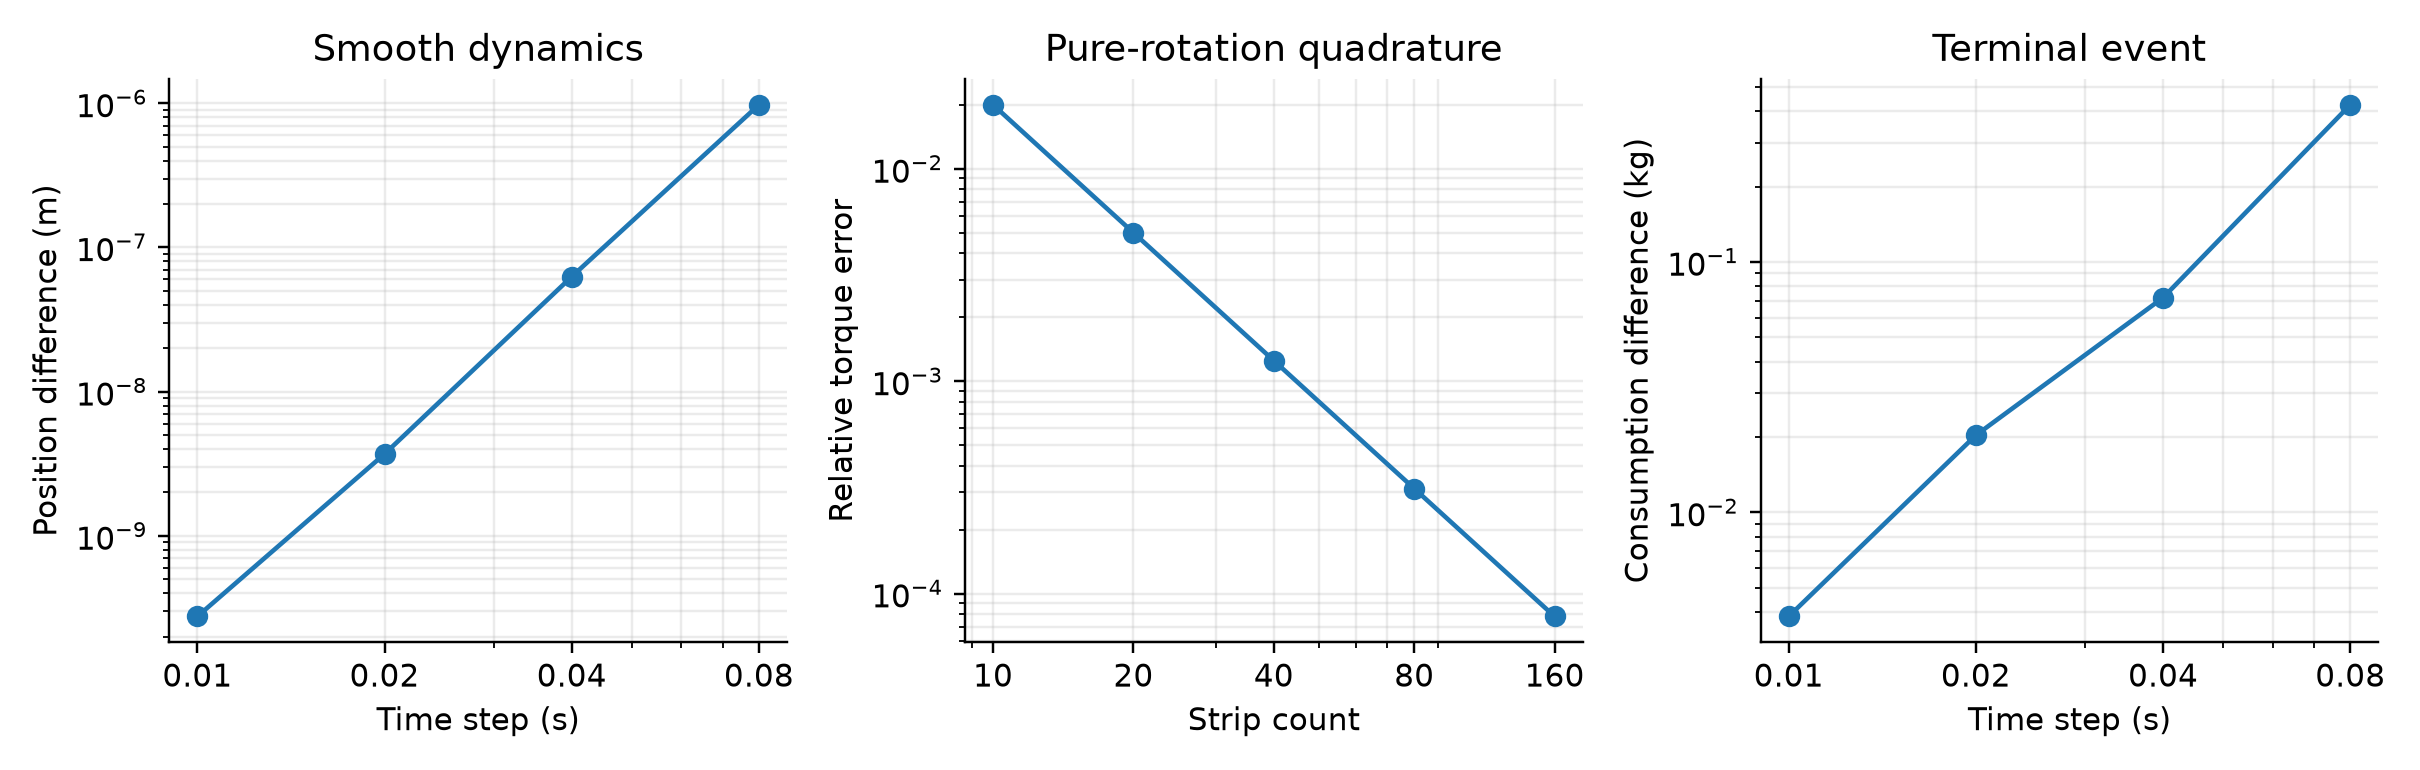
\includegraphics[width=\linewidth]{figure/p1-convergence.png}
\caption{Independent numerical error sources. Left: smooth-trajectory position difference relative to a finer same-model integration. Middle: strip torque error against the analytic integral. Right: contact-consumption difference relative to the 0.005 s run.}\label{fig:convergence}
\end{figure}
The reference implementation and P1 checks are reproducible with \texttt{node src/verify-p1.mjs}. The remaining limitations are model-form uncertainty, actuator idealization, atmosphere range, local-plane/rotation approximations, and absent structural/thermal allowables. Whole-flight feasibility and fuel optimization are delegated to the next stage.
